\section{Модули для обработки и визуализации данных}
С помощью предыдущего введения мы смогли сгенерировать необходимые данные и текст, но в настоящее время все данные и текст находятся в одном файле \textbf{\$\$pt4dat\$\$.dat}. Чтобы облегчить последующие манипуляции и визуализацию, мы также разработали два модуля \textbf{udata} и \textbf{uprint}.
\subsection{Обработка данных}
В модуле \textbf{udata} предусмотрен ряд функций для обработки данных и текста.
\subsubsection{Загрузка данных и создание файлов данных}
Функция \textbf{LoadData} считывает данные и текст из файла \textbf{\$\$pt4dat\$\$.dat} и сохраняет их в переменных.

\lstset{language=c++}
\begin{lstlisting}
void CreateAddFiles()
{
    std::ofstream f("ut1inf.dat");
    f << "11" << std::endl;             // Taskbook version
    f << cursize << std::endl;          // number of processes
    f << NumberOfUsedData << std::endl; // number of used data (in the process 0);
    f.close();

    for (int i = 0; i <= 100; i++)
    {
        if (std::filesystem::exists("ut1in" + std::to_string(i) + ".dat"))
        {
            std::filesystem::remove("ut1in" + std::to_string(i) + ".dat");
        }
        if (std::filesystem::exists("ut1out" + std::to_string(i) + ".dat"))
        {
            std::filesystem::remove("ut1out" + std::to_string(i) + ".dat");
        }
        if (std::filesystem::exists("ut1err" + std::to_string(i) + ".dat"))
        {
            std::filesystem::remove("ut1err" + std::to_string(i) + ".dat");
        }
        if (std::filesystem::exists("ut1sh" + std::to_string(i) + ".dat"))
        {
            std::filesystem::remove("ut1sh" + std::to_string(i) + ".dat");
        }
    }

    std::ofstream file;
    bool isOpen;
    for (int i = 0; i < cursize; i++)
    {
        isOpen = false;
        for (int j = 0; j < nidata; j++)
        {
            if (idata[j].r == i)
            {
                if (!isOpen)
                {
                    file.open("ut1in" + std::to_string(i) + ".dat");
                    isOpen = true;
                }
                file << idata[j].id << std::endl;
                switch (idata[j].id)
                {
                case 'b':
                case 'i':
                    file << std::round(idata[j].n) << std::endl; // TODO: this 'round' is dirfferent from the one in pascal
                    break;
                case 'r':
                    file << idata[j].n << std::endl;
                    break;
                case 'c':
                case 's':
                    file << idata[j].s << std::endl;
                    break;
                }
            }
        }
        if (isOpen)
        {
            file.close();
        }
    }
}
\end{lstlisting}
\textbf{CreateAddFiles} затем записывает эти данные во вспомогательные файлы, которые используются при проверке решения.

\begin{itemize}
    \item \textbf{ut1in}     - Хранение входных данных.
    \item \textbf{ut1out}    - Хранение данных, полученных в результате работы учебных программ.
    \item \textbf{ut1err}    - Хранение сообщений об ошибках.
    \item \textbf{ut1sh}     - Хранение отладочной информации для учебных программ.
\end{itemize}

\subsubsection{Проверка данных решения}
\lstset{language=c++}
\begin{lstlisting}
bool CheckAllResults()
{
    nrdata = 0;
    check_result = true;
    headerinfos.assign(cursize, "");
    odata_procs.resize(cursize);
    for (int i = 0; i < cursize; ++i)
    {
        std::vector<TData> odata_i;
        for (int j = 0; j < nodata; ++j)
        {
            if (odata[j].r == i)
            {
                odata_i.emplace_back(odata[j]);
            }
        }
        odata_procs[i] = odata_i;
        if (i == 0)
            continue;
        check_result = CheckResults(i) && check_result;
    }

    if (check_result)
        check_result = CheckResults(0);
    else
    {
        CheckResults(0);
        headerinfos[0] = WrongSolutionMsg;
    }

    return check_result;
}
\end{lstlisting}
Функция \textbf{CheckAllResults} вызывается pt4utilities и проверяет решение каждого процесса.

Функция CheckResults вызывается для проверки решения отдельного процесса. Она будет сравнивать один за другим данные, выведенные учебной программой, с данными правильного решения, если они все одинаковые, то оно правильное, если в нем разные данные, то учебная программа ошибается.

\subsection{Визуализация данных}
Визуализация данных имеет решающее значение для обеспечения хорошего интерактивного интерфейса для пользователей. Модули udata и uprint предоставляют ряд функций для достижения этой цели.

\subsubsection{Основные функции визуализации}
Эта часть была выполнена другим автором, Чжан Инцин, который построил основные рамки интерфейса программы, такие как границы интерфейса.
Далее приведен пример одной из таких функций.

\lstset{language=c++}
\begin{lstlisting}
// print header info
void PrintHeader(const std::string RunInfo)
{
    std::vector<std::string> s(2);
    std::string s1 = InitString(' ');
    std::string s0 = InitString(box_drawings::LIGHT_HORIZONTAL);
    PrintCmt(s0, GrTopic + std::to_string(TaskNumber) + " [" + GrDescr + "] ", 4);
    PrintCmt(s0, '(' + std::to_string(TestNumber) + ')', 75);
    s[0] = s0;
    std::cout << theme_bg << border_color << box_drawings::LIGHT_DOWN_AND_RIGHT << s[0]
              << box_drawings::LIGHT_DOWN_AND_LEFT << colors::RESET << std::endl;
    s[1] = s1;
    PrintCmt(s[1], RunInfo, 2);
    std::string bg_color = check_bg(RunInfo);
    std::cout << theme_bg << border_color << box_drawings::LIGHT_VERTICAL << bg_color << colors::WHITE << s[1]
              << colors::RESET << theme_bg << border_color << box_drawings::LIGHT_VERTICAL << colors::RESET << std::endl;
}
\end{lstlisting}
Функция \textbf{PrintHeader} используется для печати заголовочной информации интерфейса. 

Чтобы добиться эффекта непрерывной границы, мы используем для печати границ кодировку Unicode, определенную в заголовочном файле \textbf{box\_drawing}.

Функция PrintCmt определена и реализована в uprint, и она гарантирует, что каждая строка вывода на терминал будет одинаковой длины.


\subsubsection{Обработка цвета}
Чтобы сделать интерфейс более эстетически приятным, цвета всего интерфейса были тщательно обработаны.

Сначала мы разделим все цвета в интерфейсе на цвет фона, цвет границы, цвет текста и цвет данных.

\lstset{language=c++}
\begin{lstlisting}
std::string Colorize(const std::string &text)
{

    std::regex special_pattern(R"(\s*(\d+)\|\s*(\d+)\>\s*(.*))");
    if (std::regex_match(text, special_pattern))
    {
        return text;
    }

    std::regex pattern(R"((-?(true|false|\d+(\.\d+)?)))");

    std::string colored_text = std::regex_replace(text, pattern, colors::RESET + theme_bg + data_color + "$&" + colors::RESET + theme_bg + text_color);

    return ProcessString(colored_text);
}
\end{lstlisting}

Функция \textbf{Colorize} используется для установки цвета данных, где регулярное выражение используется для поиска данных, цвет которых необходимо изменить.

\begin{itemize}
    \item \textbf{theme\_bg} - Определяет ASCII-код для цвета фона.
    \item \textbf{text\_color} - Определяет ASCII-код цвета текста.
    \item \textbf{data\_color} - Определяет ASCII-код цвета данных.
    \item \textbf{border\_color} - Определяет ASCII-код для цвета границы.
\end{itemize}

Функции, используемые для вывода остальной части интерфейса, также используют коды ASCII для указания всех цветов. Эти цвета определяются перед сгенерированным интерфейсом и позволяют пользователю настраивать эти цвета.

Чтобы реализовать функцию пользовательского цвета, мы добавили файл конфигурации \textbf{config.yml}.

\lstset{language=bash}
\begin{lstlisting}
# This is a configuration file for the app's colors.
# The file specifies the RGB values for each of the five colors used in the app.

# Define the RGB value for the background color.
theme_bg: [0, 0, 50] # Black

# Define the RGB value for the data color.
data_color: [255, 255, 200] # Yellow

# Define the RGB value for the text color.
text_color: [128, 128, 200] # Gray

# Define the RGB value for the border color.
border_color: [255, 255, 255] # White
\end{lstlisting}

Перед созданием интерфейс программа считывает RGB-коды для этих цветов из этого профиля. Затем эти значения присваиваются соответствующим цветовым переменным.

\begin{figure}[htbp]%
    \centering
    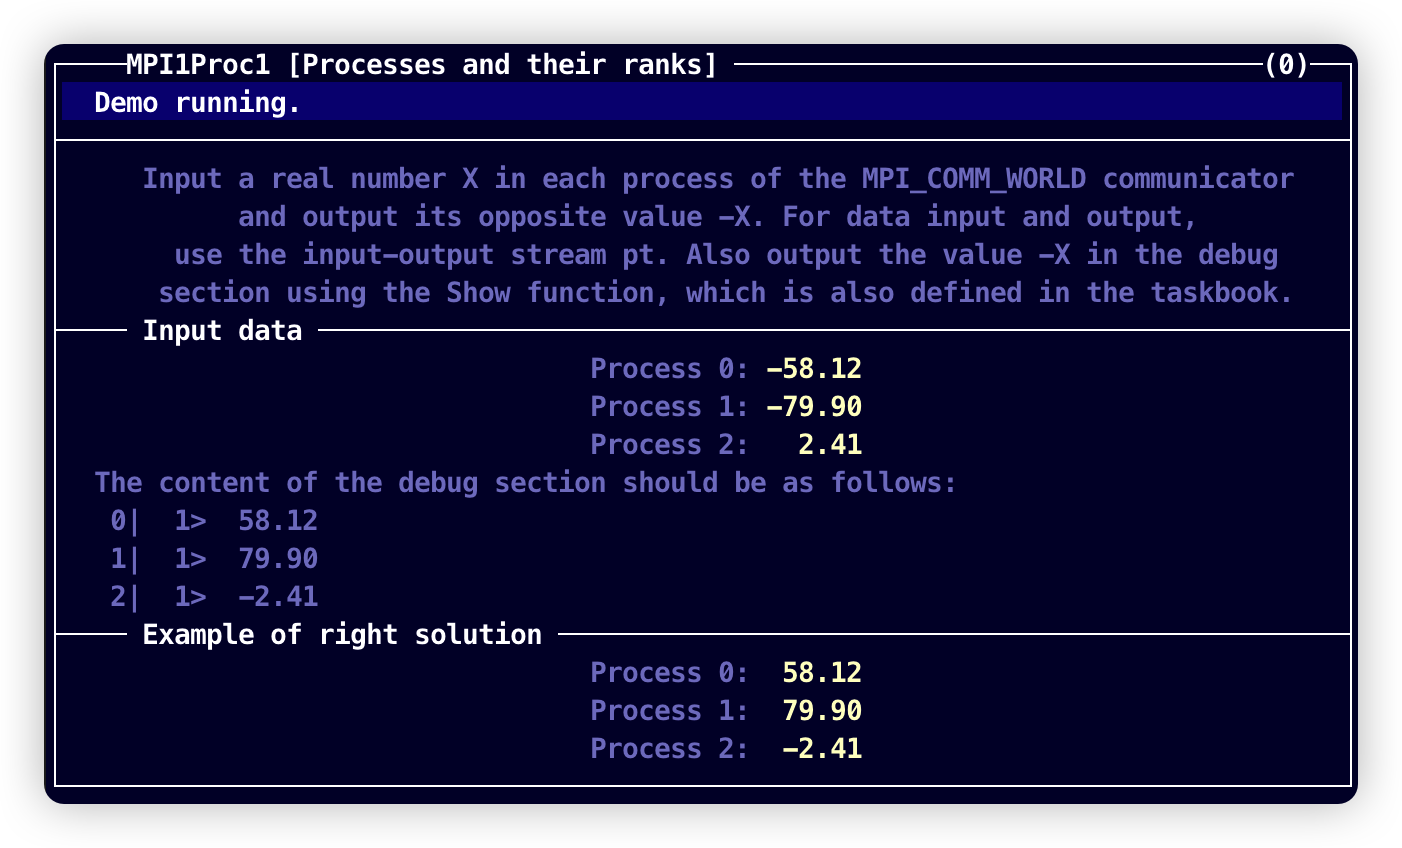
\includegraphics[width=0.9\linewidth]{images/color_example.jpg}%子图文件名
    \caption{Примеры тем.}%总标题
    \label{theme}%总标签
\end{figure}

Это изображение\ref{theme} демонстрирует эффект, достигаемый с помощью данного профиля.

Однако следует отметить, что если вы хотите, чтобы пользовательская тема вступила в силу, необходимо добавить параметр \textbf{-c custom} после команды unixTaskbook в файле \textbf{runtest.cmd}.

